\documentclass[oneside,openright]{book}
\usepackage{listings}
\usepackage{underscore}
\usepackage[breaklinks]{hyperref}
\usepackage{url}
\usepackage{breakurl}
\usepackage{graphicx}
\usepackage{atbegshi}% http://ctan.org/pkg/atbegshi
\AtBeginDocument{\AtBeginShipoutNext{\AtBeginShipoutDiscard}}
\renewcommand\thesection{\arabic{section}}
\renewcommand{\bibname}{References}
\lstset{ %
   language=C++,                % choose the language of the code
   basicstyle=\small,        % the size of the fonts that are used for the code
   keywordstyle=\color{blue},
   stringstyle=\color{red},
   commentstyle=\color{green},
   numbers=left,                   % where to put the line-numbers
   numberstyle=\footnotesize,      % the size of the fonts that are used for the line-numbers
   stepnumber=1,                   % the step between two line-numbers. If it is 1 e ach line will be numbered
   numbersep=5pt,                  % how far the line-numbers are from the code
   backgroundcolor=\color{white},  % choose the background color. You must add \usep ackage{color}
   showspaces=false,               % show spaces adding particular underscores
   showstringspaces=false,         % underline spaces within strings
   showtabs=false,                 % show tabs within strings adding particular unde rscores
   frame=single,           % adds a frame around the code
   tabsize=2,          % sets default tabsize to 2 spaces
   captionpos=b,           % sets the caption-position to bottom
   breaklines=true,        % sets automatic line breaking
   breakatwhitespace=false,    % sets if automatic breaks should only happen at whitespace
   escapeinside={\%*}{*)}          % if you want to add a comment within your codey
   }
\hypersetup{
    bookmarks=false, % show bookmarks bar?
    pdftitle={Software Requirement Specification}, % title
    pdfauthor={Malcom Diller, Evan Steele, Sean Rettig}, % author
    pdfsubject={Raspberry Pi Outdoor Lighting}, % subject of the document
    pdfkeywords={TeX, LaTeX, graphics, images}, % list of keywords
    colorlinks=true, % false: boxed links; true: colored links
    linkcolor=blue, % color of internal links
    citecolor=black, % color of links to bibliography
    filecolor=black, % color of file links
    urlcolor=blue, % color of external links
  %linktoc=page % only page is linked
}
\def\myversion{1.0 }
\title{
	\flushright
		\rule{16cm}{5pt}\vskip1cm
		\Huge{MIDTERM REPORT}\\
	for\\
		\vspace{2cm}
	Not Exactly the Internet of Things for Outdoor Lighting\\
		\vspace{2cm}
	\LARGE{Progress Report:}
	\vspace{2cm}
	\LARGE{Alpha Stage\\}
	\vspace{2cm}
	Malcolm Diller, Sean Rettig, and Evan Steele\\
        Client: Victor Hsu\\
        OSU CS Senior Capstone Group 22
		\vfill
		\rule{16cm}{5pt}
}

\date{}
\usepackage{hyperref}
\renewcommand{\contentsname}{PiLight}
\begin{document}
\pagenumbering{gobble}
\maketitle
\tableofcontents
\newpage
\pagenumbering{arabic}
\section{Abstract}

The system will consist of a wireless network of tiny ``client'' computers that
each control up to 4 sets of lights and are controlled by a central ``server''
computer, which will automatically send out commands to the clients when it's
time to turn on or off.  The central node will run a control program that can
be easily accessed via a touch screen, a web browser, or a mobile device, where
the user can locally or remotely control each light individually. The control
interface will allow users to easily set ``rules'' for what their lights do and
when, depending on the time of day, the sun/moon position, and potentially even
triggers such as weather conditions or calendar dates.\\

Through the last term and a half, our team moved through the concepts, the
documentation, and have produced an alpha-level deliverable for the project.
With regular communication through email and IRC, our group kept coordinated
throughout the term, publishing progress reports to the Sharepoint site and
code samples to our Github page. We will discuss our weekly progress and
describe how the prototype and documentation unfolded over the course of the
first term of the capstone project. This should provide an assessment on where
our groups stands in preparedness to move forward with increased functionality
in preparation for a beta presentation.

\pagebreak

\section{Status}

At this point in the project, all alpha-level features have been implemented;
all planned user interface pages and their corresponding elements have been
created and at least stubbed; not all elements are fully functional yet.
However, many of the elements are already at beta-level functionality:

\begin{itemize}
    \item The ESP firmware has been written and can automatically connect to
        the Pi wirelessly. \\ \\
      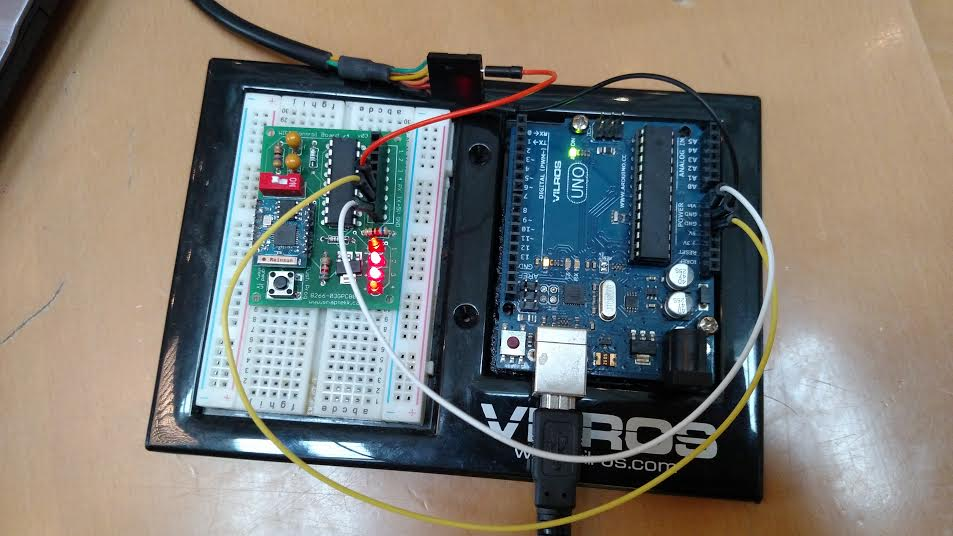
\includegraphics[width=1.0\textwidth]{pi-esp.png}
    \item The Pi is loaded with our custom build of Yocto Linux and can act as
        a wireless router for the ESPs to connect to. \\ \\
      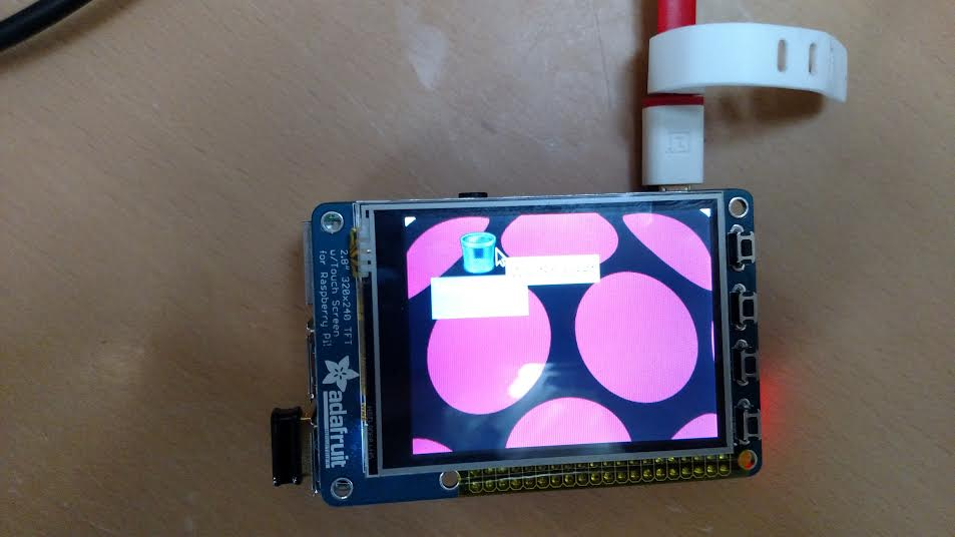
\includegraphics[width=1.0\textwidth]{pi-screen.png}
    \item The Pi is set up to run our Flask web site, and it can be connected 
        to by wireless devices and viewed in a browser.
    \item The Flask web site has a SQL database that stores information about
        the lights, groups, devices, rules, and users.
    \item The web interface has a main page that lists all available lights,
        where lights can be renamed and sorted into groups. \\ \\
      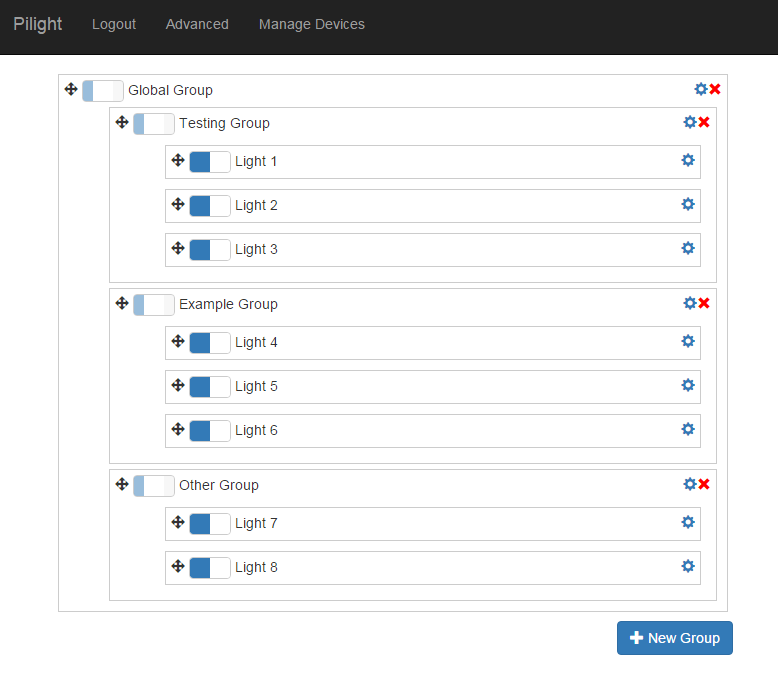
\includegraphics[width=1.0\textwidth]{main-page.png}
    \item Groups in the main page can also be created, renamed, nested into
        each other, and deleted, though deletion has not been fully implemented
        yet.
    \item The web interface has an advanced page for each light/group where
        rules for when to automatically toggle on/off can be created.
    \item All types of rules (including time of day, day of week, day of month,
        day of year, specific dates, sunrise/sunset times, and even parent
        interaction and offsets/staggering) are available to be created. \\ \\
      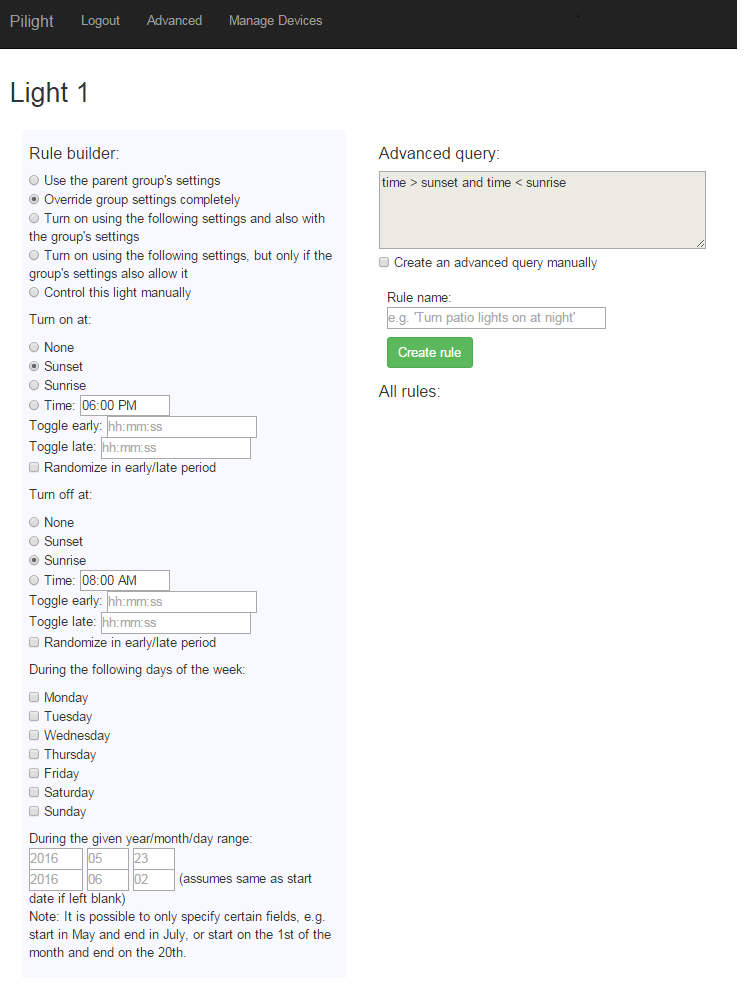
\includegraphics[width=1.0\textwidth]{advanced-page.png}
    \item The web interface has a login screen. \\ \\
      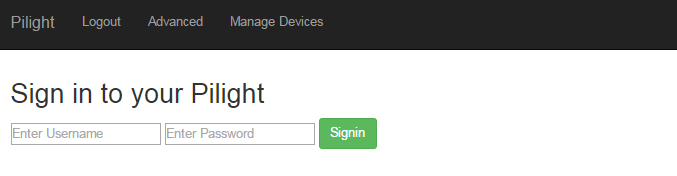
\includegraphics[width=1.0\textwidth]{login-page.png}
    \item The web interface has a device pairing screen. \\ \\
      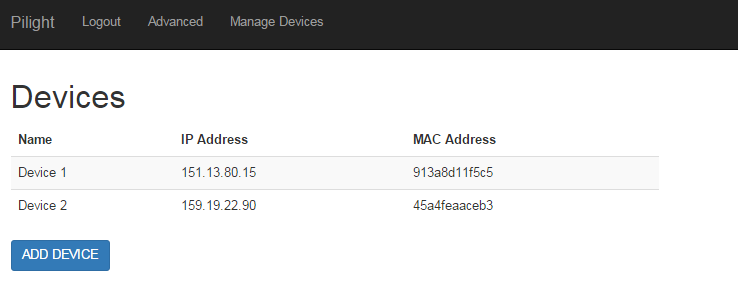
\includegraphics[width=1.0\textwidth]{devices-page.png}
\end{itemize}

\section{Work in Progress}

\subsection{Device Communication}

One of the current post-Alpha goals is to complete the communication mechanism
between the Raspberry Pi and the ESP8266 modules. We are working on finalizing
our logical evaluation subsystem and determining what do to in the case of
manual user override. The databases and communication parameters have been
completed; we know what the function that will flip the lights themselves
expects, but we don't know how to perform our Python-based evaluations yet. We
expect that it will come shortly after finishing up the advanced query editor,
at which point we expect to have a format and value range locked down for the
queries to be evaluated.\\

The devices are already prepared in a database to draw from, using the MAC
address as the unique key to locate the IP address from the table. We don't
anticipate the ISC DHCP server flipping addresses around, but by using the
physical hardware addresses we are eliminating any possibility of sending the
code to the wrong device. The Python ISC DHCP library provides us with a
mechanism for determining if a device's IP has changed, and we will write that
change to the devices table.

\subsection{User Interface/Website}

Much of the functionality that we need for Beta has already been completed.
The database has been created and the main page is currently able to persist
user-submitted data, such as the names of groups and lights.  The advanced page
has yet to actually perform any server communication for persistence of
user-submitted data, but the implementation of this will be similar to the
front page.  There are also a few UI elements that are currently not
implemented, such as group deletion on the main page, but none of these require
new knowledge in order to implement and should be completed soon.

\subsection{Scheduling System}

The scheduling system is what ties together the website with the hardware
communication; it periodically evaluates all rules for all lights/groups and
initiates the sending of signals to the ESP8266 modules based on which lights
are to be turned on/off.  The scheduling system is also in charge of parsing
the group/light rules that are stored in JSON format into boolean logic
expressions that can be evaluated, including replacing keywords such as
"sunset" and "sunrise" with actual times based on the user's location and the
time of the year.  So far, the basic JSON to boolean expression conversion has
been implemented.

\section{Problems}

\subsection{Wireless}

We had an issue early on with how we planned to connect to the ESP8266 modules
using our Raspberry Pi. Our proof-of-concept had the client connecting to the
wireless module itself to make changes, but we wanted remote management to work
from the Pi and have it be reachable from the internet. We began looking into
ways to perform local routing so that the device could play with the end user's
home network, but ran into more snags trying to configure multiple wireless
network devices on the same Pi. We contacted our client, who suggested that we
not worry about external connectivity for the project. His expectations were
that users would directly connect to the Pi to make configuration changes. The
project title was "not \textit{exactly} the Internet-of-Things", after all.\\

To fix the issue, we reconfigured the Raspberry Pi so we could connect
wirelessly. We needed to first recompile \textit{hostapd} to run with a version
of our USB wireless driver that could broadcast an SSID. After recompiling, we
confirmed that we could connect using a wireless device, such as a smartphone.
The other task was to change the firmware on the ESP8266 so that it behaves
like a client instead of a host. In addition to flashing the new firmware, a
startup file was added so that it automatically connects to the nearest
Raspberry Pi with "Pilight" in the SSID. We will likely change this later to
better incorporate new devices.

\subsection{Pulse Width Modulation}

We had the idea that a device managable via the Raspberry Pi would be able to
control the brightness of the lights using PWM. Unfortunately the 10A gates on
our relay just can't flip fast enough for any desired pulses. Our group
contacted our client to see if it was worth the trouble of acquiring a relay
unit that could do PWM, but his response was that he was only concerned with
turning the devices on and off. We also considered a software-defined PWM
solution, but were again affected by the speed of the relay itself not being
sufficient.

\subsection{Behavior of On/Off Switches}

Before starting to implement the rules, we had not put much thought into what
the behavior should be for the On/Off switches of the lights and groups. After
we began to implement more of the project, we realized that there are a few
ways that the behavior could be implemented:

\begin{enumerate}
  \item Toggling the switch would change the state of the light until the user
      chose to resume automated control.
  \item Toggling the switch would change the state of the light for a preset
      amount of time before resuming automated control.
  \item Toggling the switch would change the state of the light until the next
      time that the rules determined the light should change, upon which
      automated control would resume.
\end{enumerate}

The are benefits to each implementation and it was a difficult decision to
figure out which path we should take. The first option makes sense because the
user is never overridden by the system. The second option is useful because the
user most likely is turning on the light for a temporary purpose, and probably
will not want to have to go into the advanced settings all the time. We decided
to go with the third option, as it provided the benifits of the second option,
but more cleanly eases back into the pattern of automated control.  However,
this solution does require extra state tracking on the server side to know when
a light is being toggled by the re-evaluation of a rule, as the original design
was to have the rule evaluation happen independently of the current state of
the light.

\section{Code}

\subsection{Acquire New Devices}

This code, upon user request, scans currently connected devices for a new
ESP8266 device that does not already exist in the devices database.

\begin{lstlisting}
   // Get all DHCP leases currently given out
   leases = IscDhcpLeases('/var/lib/dhcp/dhcpd.leases')
   leases = leases.get()

   // No DHCP leases at all, the server is not operating
   if not leases:
      return "NODHCP"

   additions = 0
   // For each lease, first see if it is an ESP8266
   for iteration,lease in enumerate(leases):
      if(ESP8266_check(lease.ip)):
      // We have an ESP8266 mode!
         database_check = model.Device.query.filter_by(mac=lease.ethernet).first()
         if database_check is None:
         // We have an ESP8266 AND it is not in the database!
            new_device = model.Device(mac=lease.ethernet,ipaddr=lease.ip,name="ESP8266@"+lease.ethernet)
            model.db.session.add(new_device)
            model.db.session.commit()
            additions = additions + 1
      return str(additions)
   \end{lstlisting}

\subsection{Editing Lights and Groups}

We decided to use the X-editable library for executing inline edits to the
names of groups and lights. This involved creating a span element to represent
the name with information about the light or group embedded in it. We then
included a few lines of JavaScript to specify where to send the POST request
and set up the editable span element. When submitted, a POST request would be
sent to the Flask server. Below is the Flask function that handles the POST
request and changes the name of a light or group in the database.

\begin{lstlisting}
@app.route('/change_name', methods=['POST'])
def change_name():
    name = request.form['value']
    pk = request.form['pk']
    isLight = request.form['name'] == "light"
    if isLight:
        light = model.Light.query.filter_by(id=pk).first()
        light.name = name
    else:
        group = model.Group.query.filter_by(id=pk).first()
        group.name = name
    model.db.session.commit()
    return "Success!"
\end{lstlisting}

\section{User Studies}

\subsection{User Study A}

After exploring the interface for a time, the user was asked to perform a
series of tasks to replicate common use cases for the system, including logging
in, toggling lights/groups, renaming lights/groups, reorganizing lights/groups,
creating additional groups, connecting additional client modules to the server,
and creating advanced rules for lights/groups.

\begin{itemize}
    \item The user had no problems with the login system, but they disagreed
        with the text on one of the buttons.
        \begin{itemize}
            \item The SignIn text on the button should be changed to Sign In.
        \end{itemize}
    \item There was a slight issue with the Add Devices button, as the user was
        confused by the loading animation, and had a suggestion for how to fix
        it.
        \begin{itemize}
            \item There should be text to indicate what is going on during the
                loading animation for adding devices.
        \end{itemize}
    \item The user had no problems changing the name of a light.
    \item The user was able to correctly identify that the group/light system
        was a heirarchy where lights were owned by groups and groups were owned
        by parent groups.
    \item The user was able to toggle the light on and off, however they
        thought that the switches were not very intuitive, and they had a few
        suggestions for improvement.
        \begin{itemize}
            \item The switches should be green/red, not blue/gray.
            \item The switches are too slow, and should be twice the speed.
            \item The switches should show "On" and "Off" text.
            \item The groups should have two on and off buttons instead of
                switches, and should not have a state. The intermediate state
                of the switch does not make sense.
        \end{itemize}
    \item The user was able to correctly identify that the red "x" was the
        intended button for deleting a group.
    \item There was a slight problem when the user attempted to move a light to
        a different group. The user identified the move icon as the correct
        tool for moving rows, but had difficulty clicking on it, as the spaces
        inbetween the arrows do not register a click. Once they had grabbed it
        and were moving it, they were then slightly confused because there was
        no preview of the destination, and instead the light was attached to
        the mouse. They did drop it and move the light correctly, but they
        noted that the task was slightly less intuitive than the previous ones.
        \begin{itemize}
            \item When dragging and dropping lights or groups, there should be
                a preview of the destination while the user is holding it.
        \end{itemize}
    \item The user had no problems adding a new group, but they disagreed with
        how the new group was set.
        \begin{itemize}
            \item When adding a new group, the switch should be set to Off.
        \end{itemize}
    \item The user was able to navigate to the advanced page for a light by
        clicking on the gear.
    \item When asked to set the light to turn on at sunset and turn off at
        sunrise, the user was able to find the correct radio buttons. The user
        then noted that they were not sure whether they needed to do anything
        else to save what they had done.
        \begin{itemize}
            \item There should be a "Save Changes" or "Submit" button
        \end{itemize}
    \item The user was able to correctly set the light to turn on at a specifig
        time of the day.
    \item The user was unable to set multiple rules, as it was not obvious to
        them how the rule system worked, they made a few suggestions for how
        the system could be improved.
        \begin{itemize}
            \item The New Rule and rules controls should be at the bottom of
                the page, and that the wording should be changed to something
                other than "Rule.".
            \item Advanced query box should be moved to bottom of page or
                hidden in something like an expanding box, as most users will
                not want to see or understand it.
            \item There should be a preview of the rules for a group or light
                when hovering over the name or the link leading to the advanced
                page.
            \item The wording "Rule" should be changed to something that
                represents the idea more clearly.
        \end{itemize}
    \item The user was able to identify the purpose of the menu bar but thought
        that it was not very noticable.
        \begin{itemize}
            \item Menu bar should have greater contrast so it is more
                noticable.
        \end{itemize}
\end{itemize}

As we conducted this user study near the end of Alpha stage, we have yet to
decide whether to implement the suggested changes and have yet to make any
changes as a result of the usability tests. We will go over these in the future
and make judgements about what changes should be made then.

\subsection{User Study B}

\begin{itemize}
    \item User had no issues with the login page.
    \item User attempted to rename a light, but clicked away when done editing
        rather than hitting enter, causing the rename to not be saved.
        \begin{itemize}
            \item Suggestion: Clicking away should also save a rename.
        \end{itemize}
    \item User noticed that it was not obvious which features were available on
        the front page.
        \begin{itemize}
            \item User suggested that a small blurb or tutorial should pop up
                on the first use that tells the user about renaming, moving,
                creating, deleting, and editing lights/groups.
        \end{itemize}
    \item User was not sure whether lights were on or off.
        \begin{itemize}
            \item User suggested that the switches should use actual "on/off"
                text and maybe more obvious colors than blue and gray.
                Possibly gray out the entire light's box if it's off.
        \end{itemize}
    \item User was not sure how to create a new group.
        \begin{itemize}
            \item User suggested that the "create group" button be made more
                obvious.
        \end{itemize}
    \item When asked to add a device to the system, the user was stumped
        because they did not notice the "manage devices" tab.
        \begin{itemize}
            \item User suggested that the area for adding devices be displayed
                more prominently.
        \end{itemize}
    \item On the advanced page, the user felt that there were too many elements
        in general.
        \begin{itemize}
            \item The user suggested that only the most basic and commonly used
                elements of the rule builder should be shown by default.  The
                more complex settings and the advanced query should only show
                up if the user clicks a "show more options" button or the like.
        \end{itemize}
    \item On the advanced page, the user found it confusing that they had to
        click the "create rule" to finalize the rule and that there could be
        multiple rules for one light.
        \begin{itemize}
            \item This could possibly be alleviated by only allowing one rule
                for each light.  This would help simplify the UI, and most
                users probably won't want multiple rules for each light anyway.
                Advanced users would still have the option to manually edit the
                advanced query in order to achieve the effect of having
                multiple rules.
        \end{itemize}
    \item The user found it difficult to edit the settings for groups of lights
        due to the clumsiness of having to navigate back to the front page in
        order to view the other lights.
        \begin{itemize}
            \item The user suggested that something like "next light" and
                "previous light" buttons or the like be added to the advanced
                page in order to improve ease of navigation.
        \end{itemize}
\end{itemize}

\subsection{User Study C}

\begin{itemize}
    \item User did not understand the multi-state light switch.
        \begin{itemize}
            \item Suggestion: Add a tooltip (maybe only for the first time?) or
                add a hover element to the button indicating the current state.
        \end{itemize}
    \item User did not understand what the group symbols meant.
        \begin{itemize}
            \item Suggestion: This one could just be "read the documentation"
                that we will include in the final project. It will probably be
                a PDF attachment or a Github wiki page.
        \end{itemize}
    \item User did not know if a custom query was running
        \begin{itemize}
            \item Suggestion: We'll add a note next to a light if it is
                currently controlled by a query. We can have a hover element to
                display the specific query.
        \end{itemize}
\end{itemize}

\newpage
\Urlmuskip=0mu plus 1mu\relax
\bibliography{design}{}
\bibliographystyle{IEEEtran}

\end{document}
